\documentclass[english]{tktltiki}
\usepackage[pdftex]{graphicx}
\usepackage{subfigure}
\usepackage{booktabs}
\usepackage{url}
\usepackage{amsthm,amssymb}
 \usepackage{amsmath}
 \usepackage{enumerate}
 
 \usepackage{chngcntr}
\counterwithin*{equation}{section}
\counterwithin*{equation}{subsection}

\begin{document}
\onehalfspacing

\title{Workshop 7}
\author{P�ter Ivanics}
\date{\today}

\maketitle

\section{Problems 1-4}
Note: the formulas are already written in with their negated forms in the scanned handwriting below.
	\begin{center}
		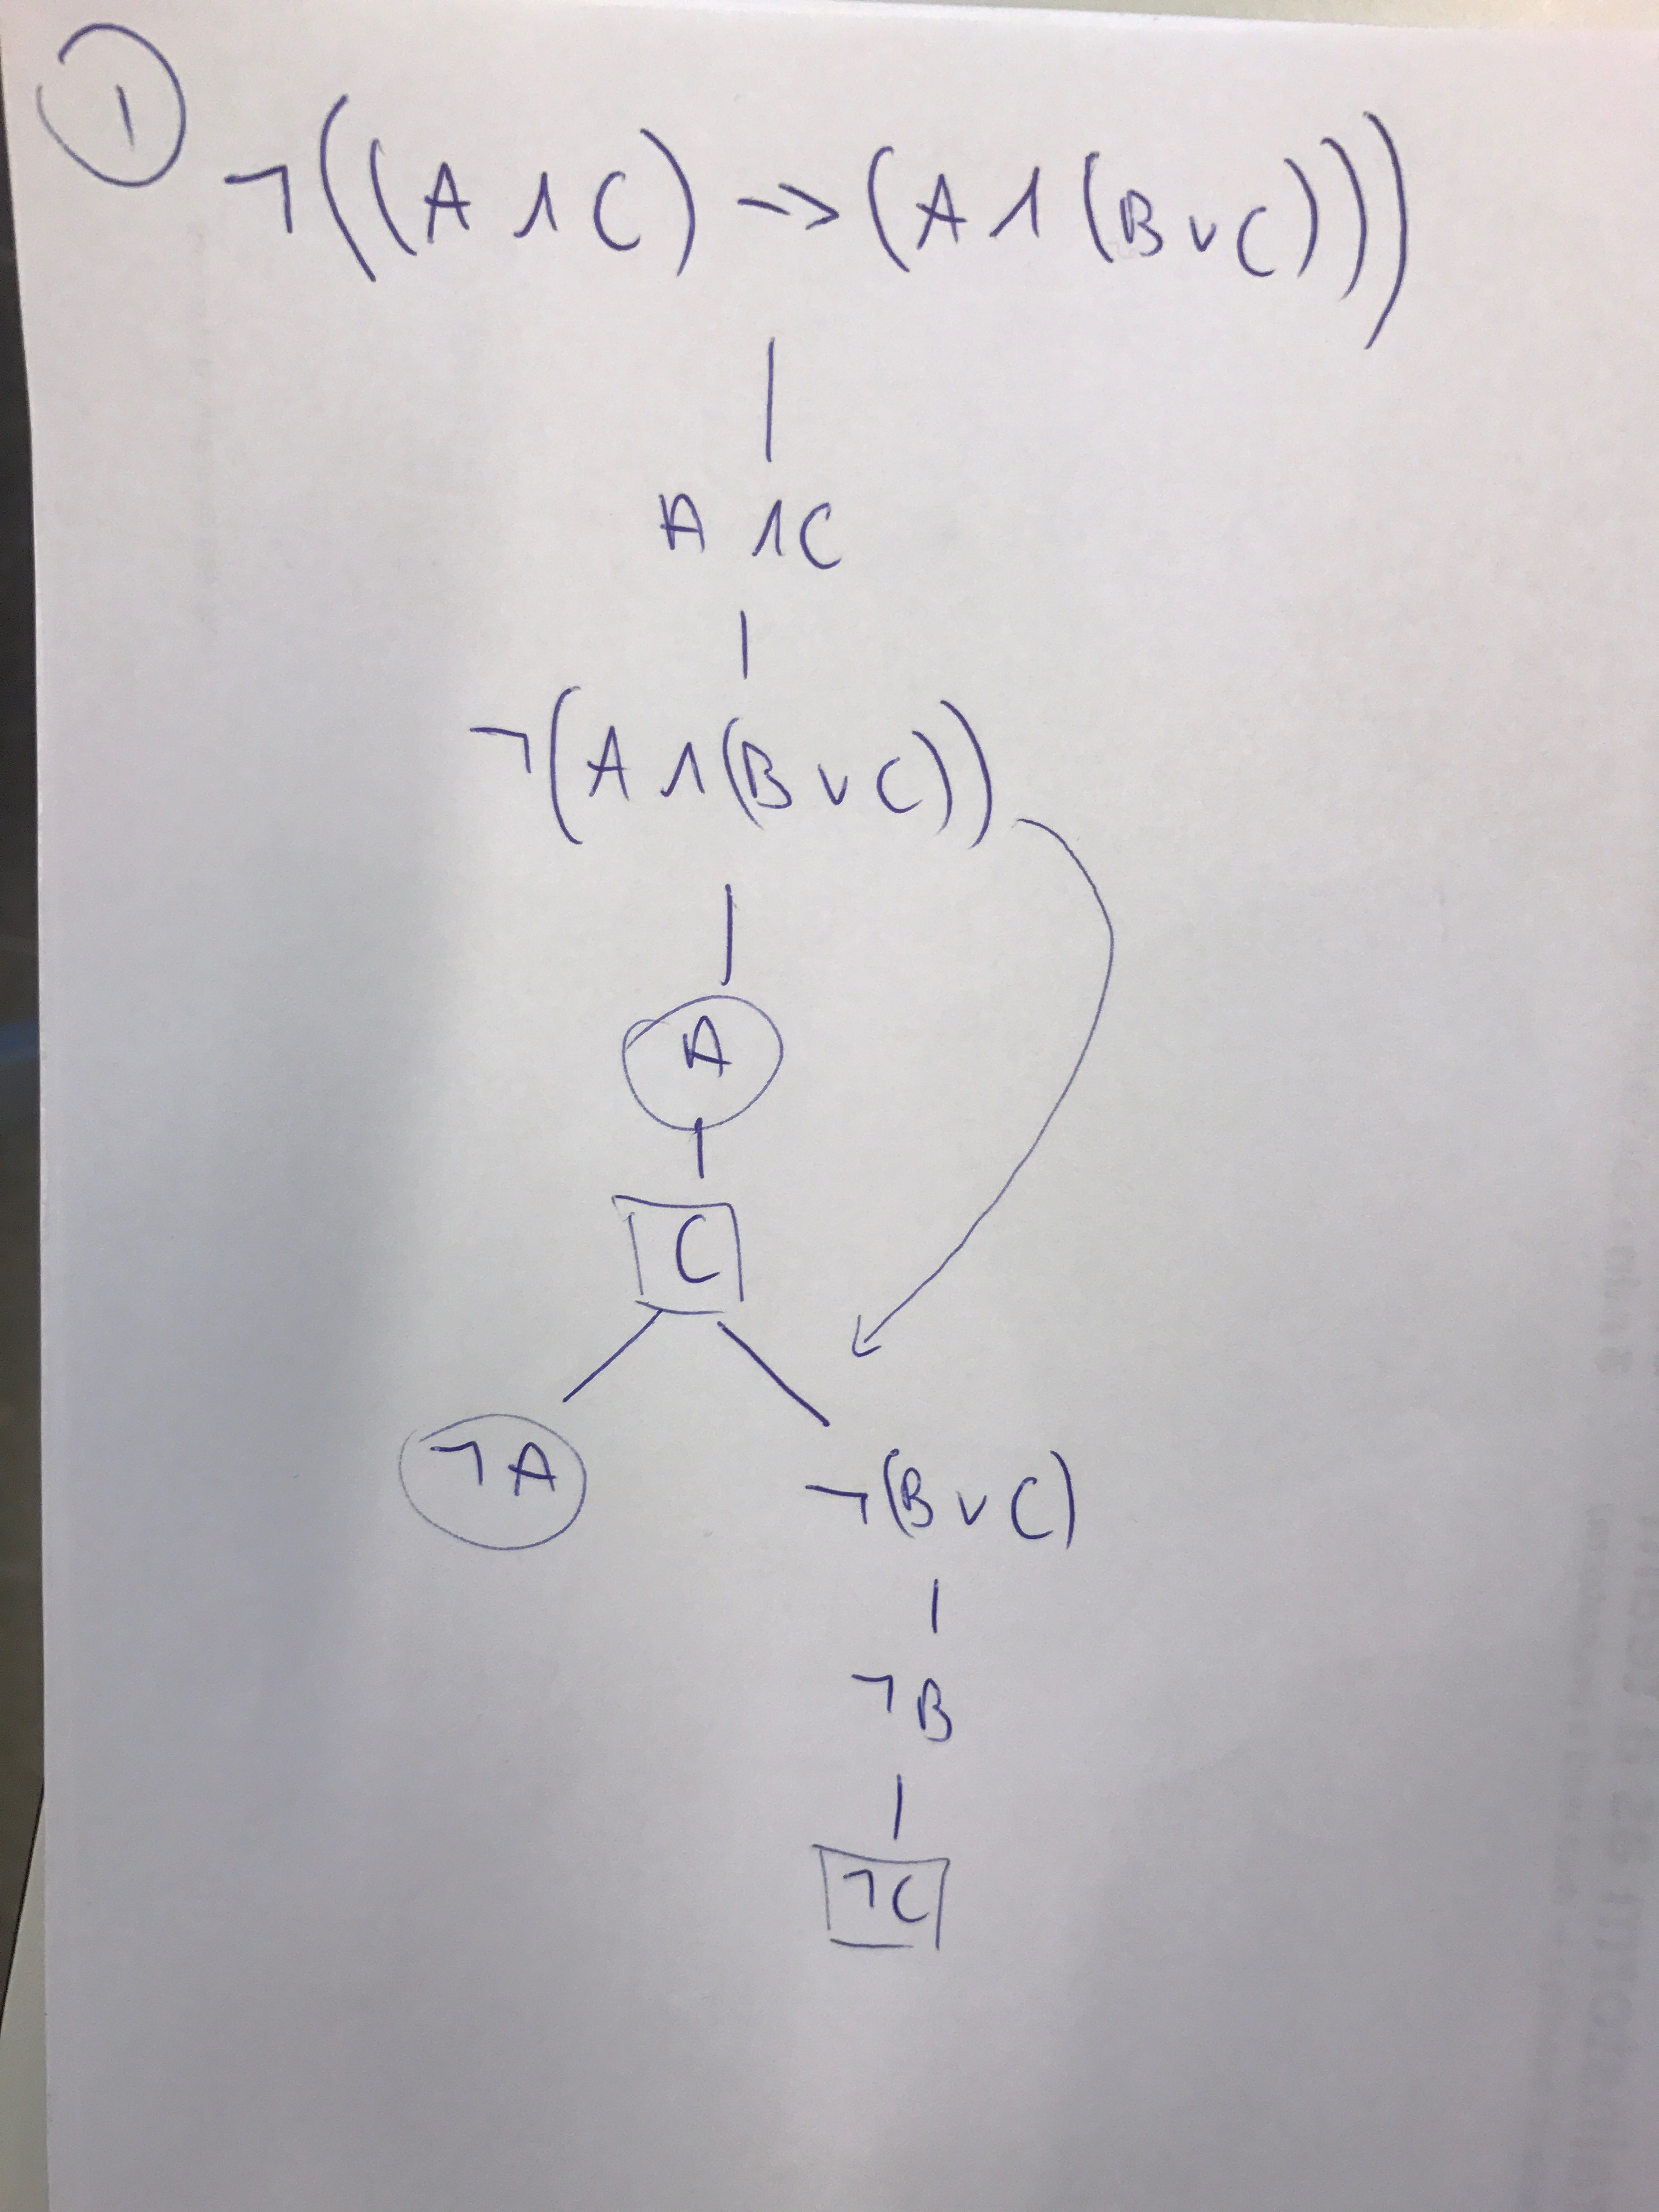
\includegraphics[width=0.5\textwidth]{images/workshop7_problem1.jpg} 
		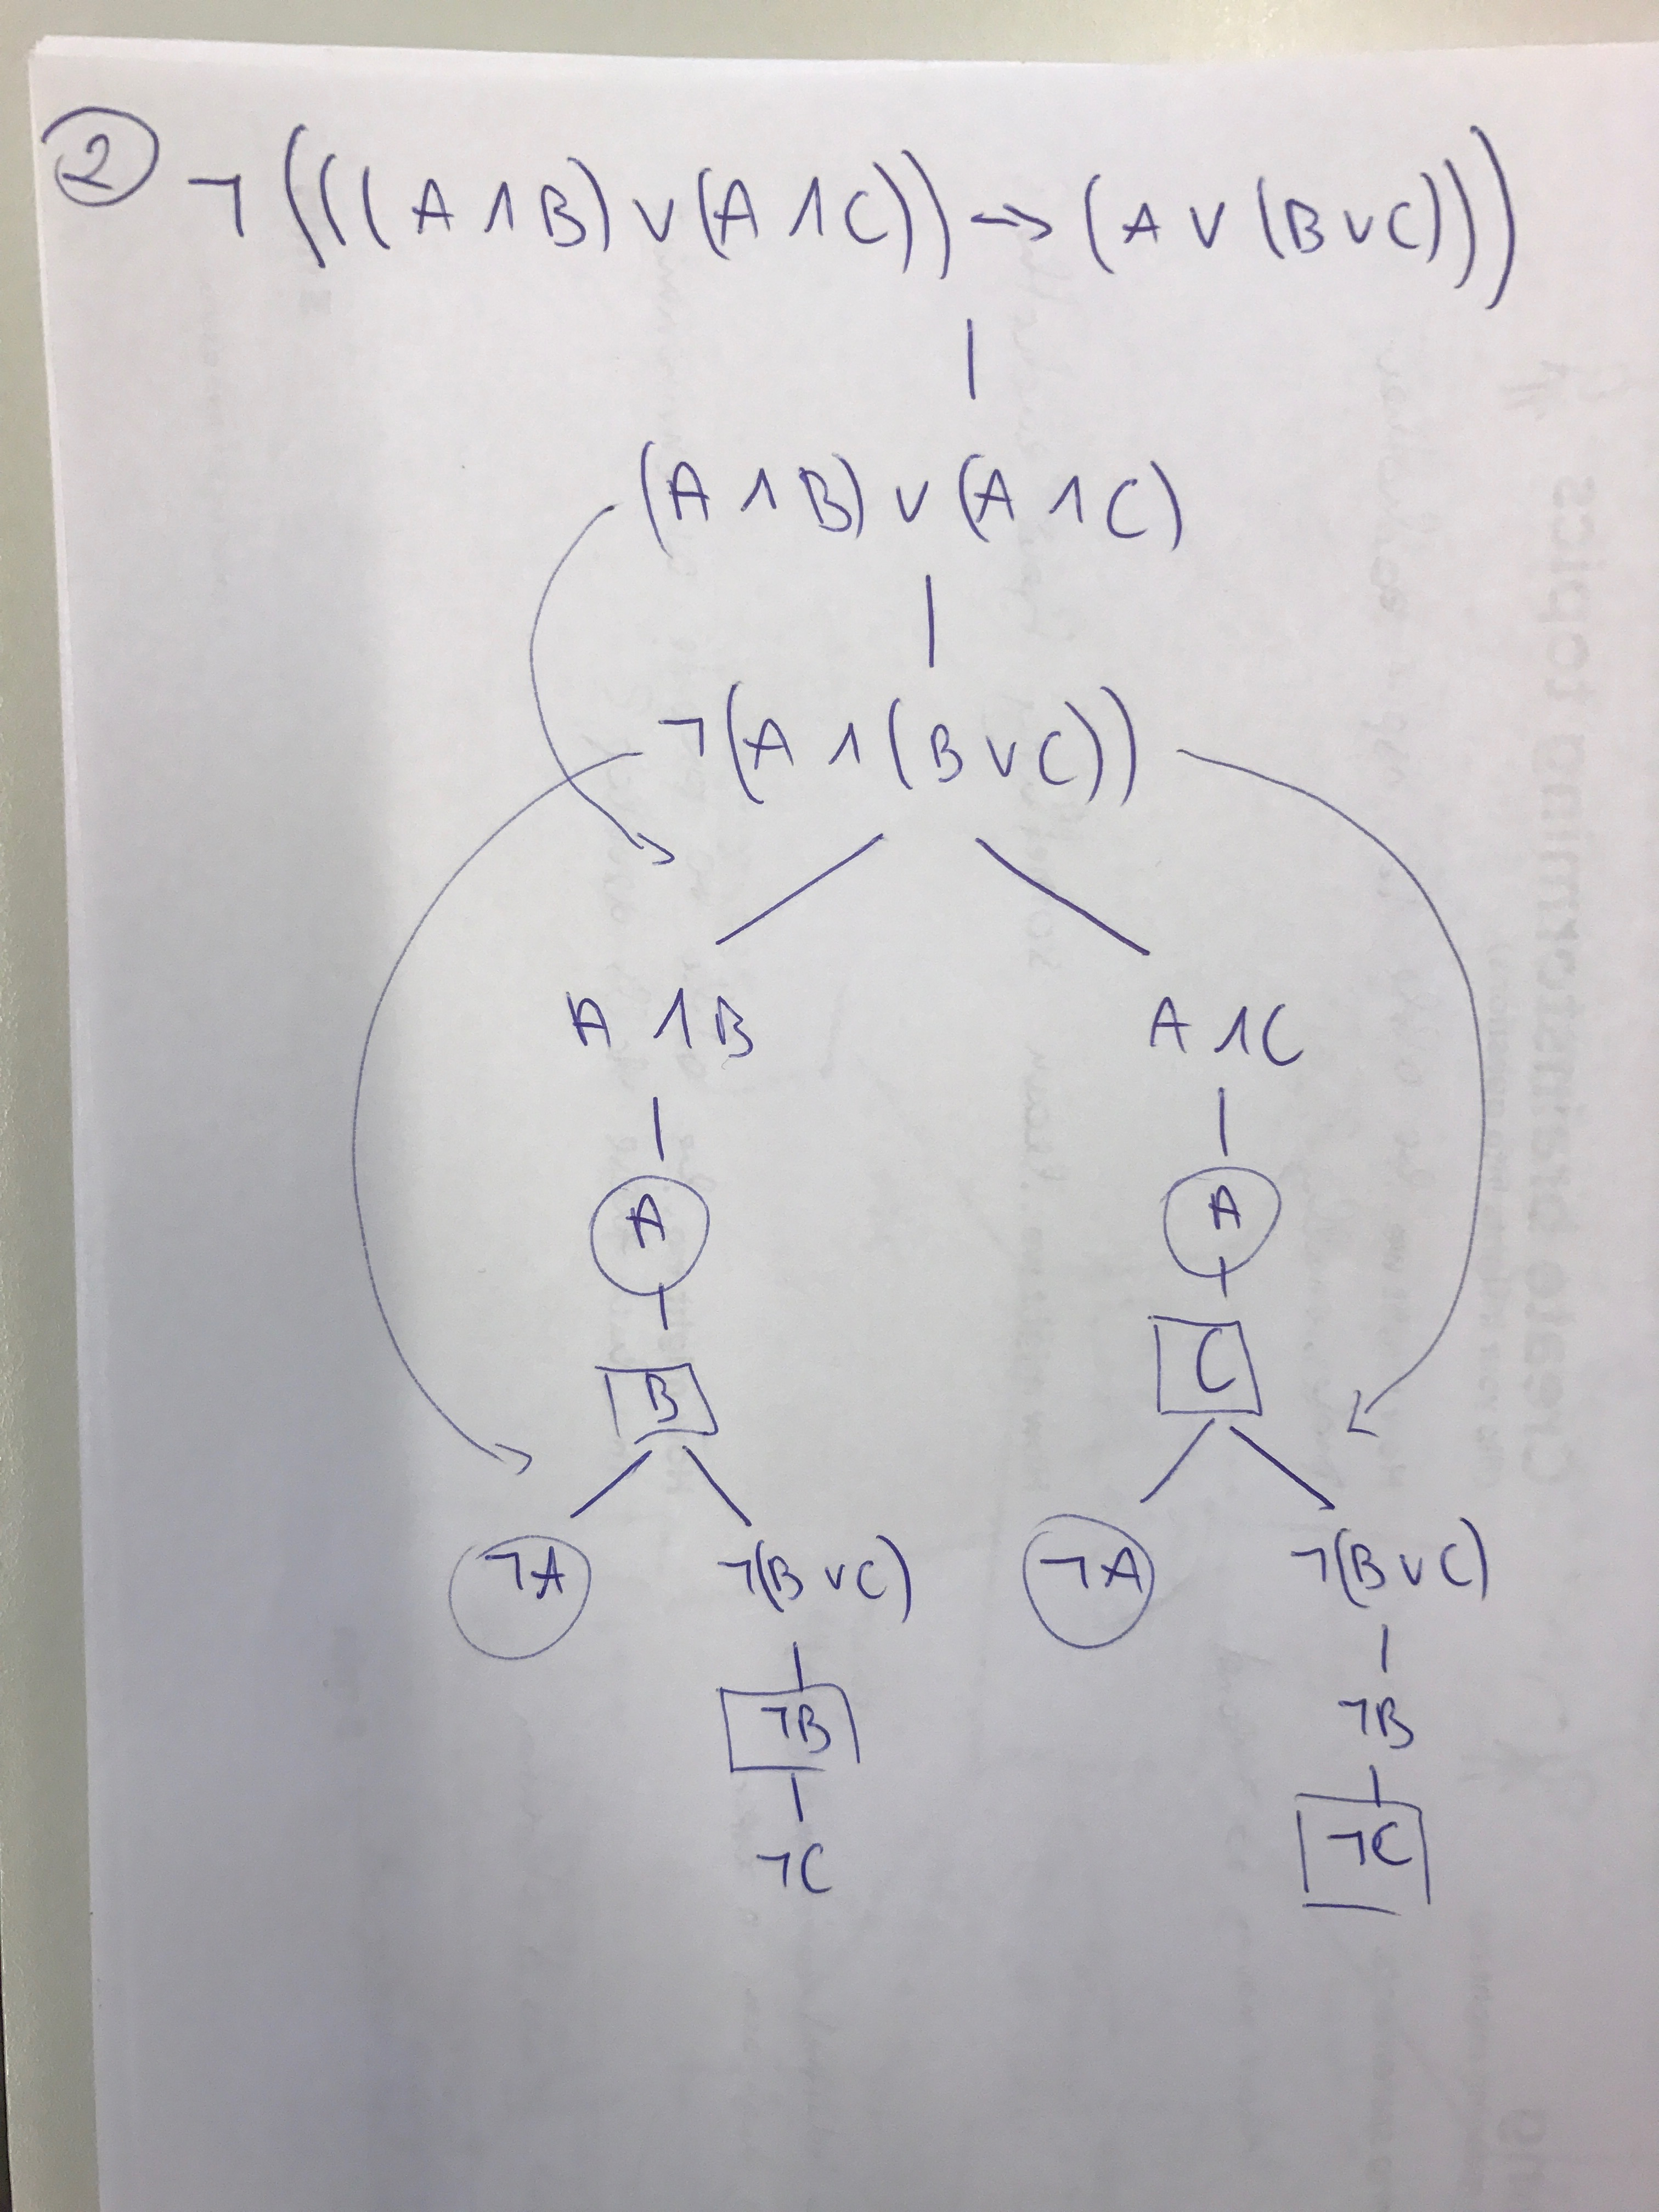
\includegraphics[width=0.5\textwidth]{images/workshop7_problem2.jpg}
		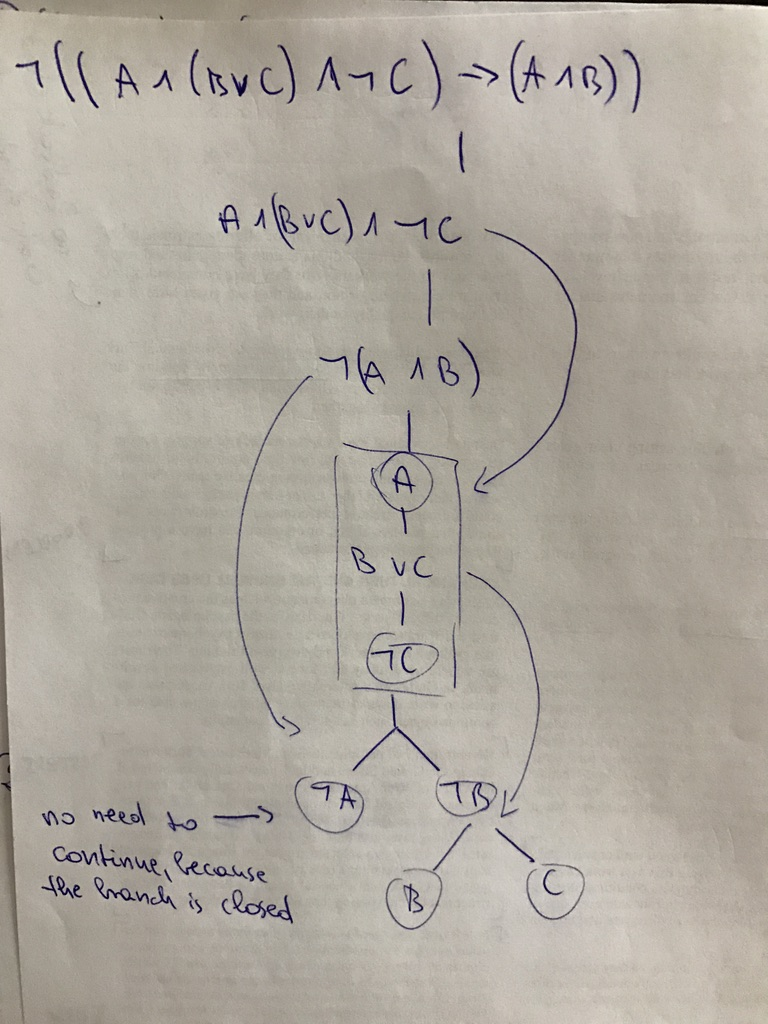
\includegraphics[width=0.5\textwidth]{images/workshop7_problem3.jpg}
		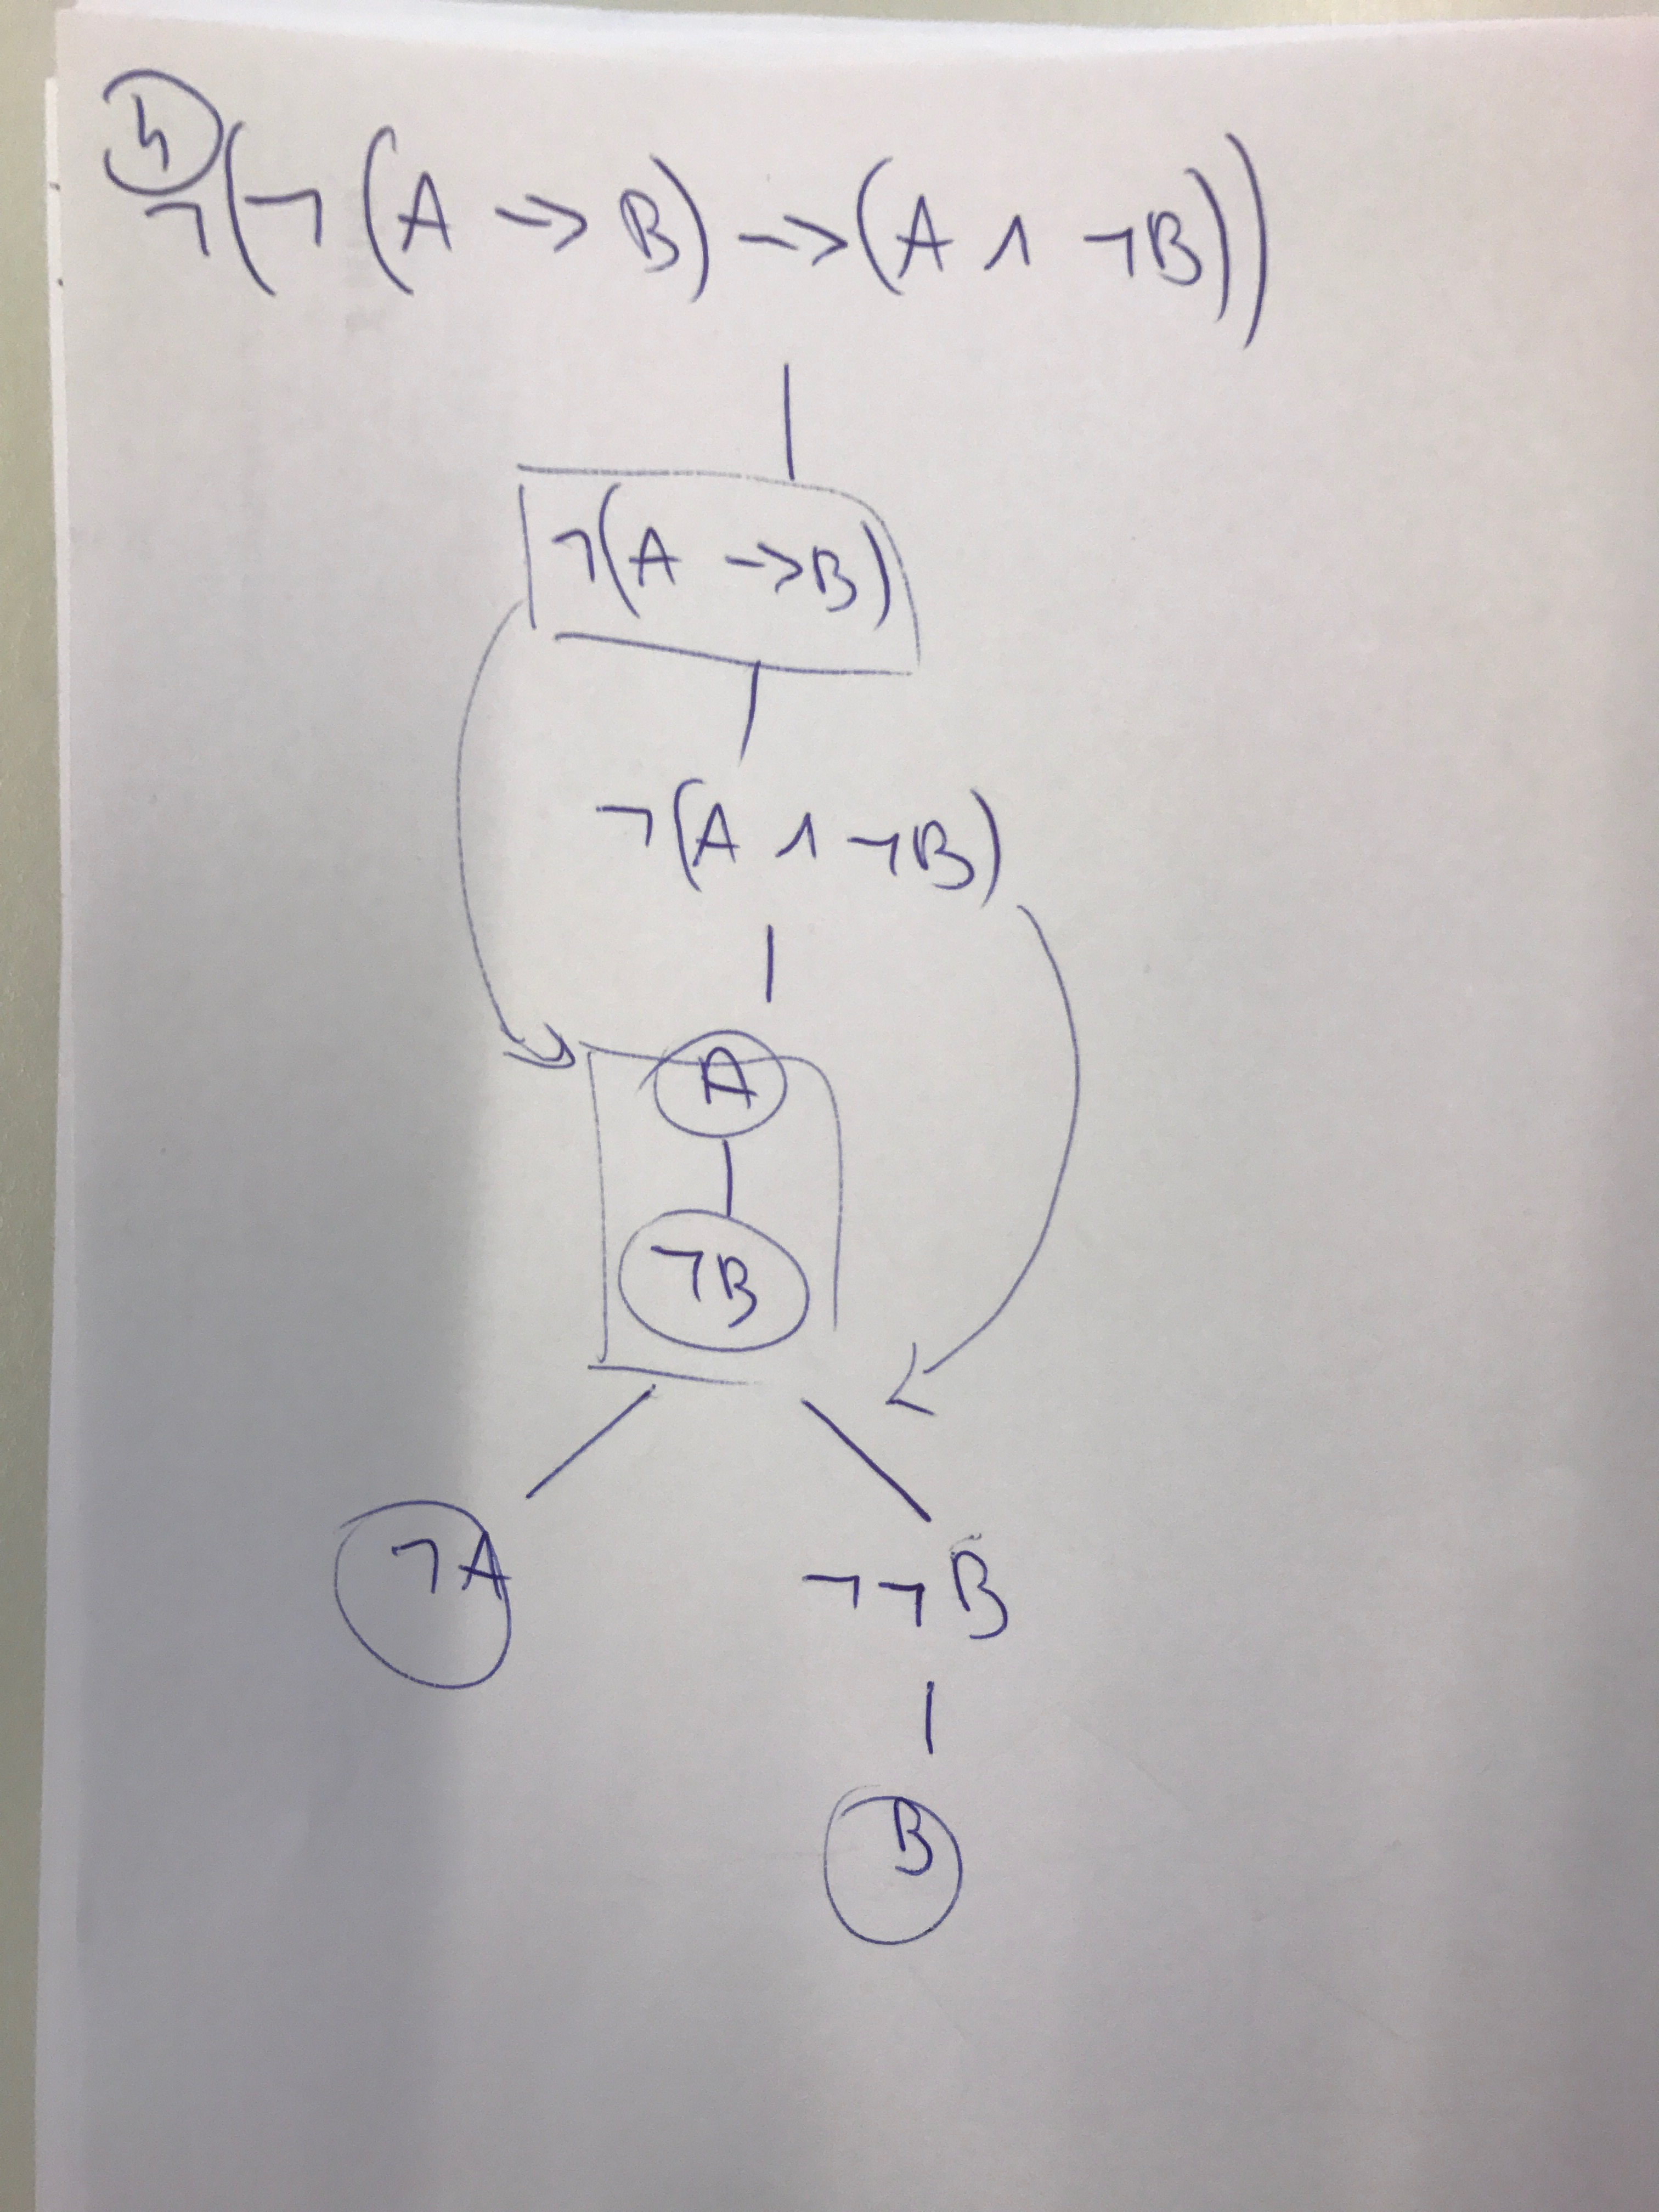
\includegraphics[width=0.5\textwidth]{images/workshop7_problem4.jpg}
	\end{center}
\section{Problem 5}
\section{Problem 6}
\section{Problem 7}
\section{Problem 8}
\end{document}